\chapterpage\chapter{Evaluation}
    In diesem Abschnitt wird anhand der SMAPE-Metrik quantifiziert, wie viel die Leistung des Modells verbessert, indem die Ausreißer durch die vorgeschlagene Methode entfernt werden, und das Ergebnisse werden diskutiert.
    
    Bevor die Leistungsänderungen des Modells für jede Methode aufgeführt werden, wird die Metrik SMAPE, die im Schritt „Evaluierung“ des Abschnitts \ref{sec:Modellierung der Feinstaubkonzentration} erwähnt wird und die ein Kriterium für die Evaluierung darstellt, ausführlich erläutert.
    
    \section*{SMAPE}
    
    \section*{Ergebnisse}

        위에서 언급한 것과 같이 훈련데이터세트와 검증데이터세트를 합친 후 데이터를 네가지 센서에 대한 데이터 세트로 만들고 다섯가지의 알고리즘을 각 데이터세트에 적용하여 이상치를 검출했습니다. 결과에 대한 시각적 정보는 그림 1에서, 결과에 대한 정량적 정보는 표 1에서 확인할 수 있습니다. 그림 1은 정보를 간략히 하기 위해 센서 'DEUS'에 대한 결과만을 다룹니다.
        Wie oben erwähnt, wurden nach dem Verschmelzen des Trainings- und Validierungsdatensatzes die Daten in vier verschiedene Datensätze für vier Sensoren aufgeteilt, und fünf Algorithmen wurden auf jeden Datensatz angewendet, um Ausreißer zu erkennen. Visuelle Informationen zu den Ergebnissen sind in Abbildung \ref{fig:Ergebnisse in 2D} und quantitative Informationen zu den Ergebnissen sind in Tabelle \ref{tab:Ergabnisse in SMAPE} zu finden. Abbildung \ref{fig:Ergebnisse in 2D} enthält der Einfachheit halber nur die Ergebnisse für den Sensor „DEUS“.

        \begin{figure}[h]
            \centering
            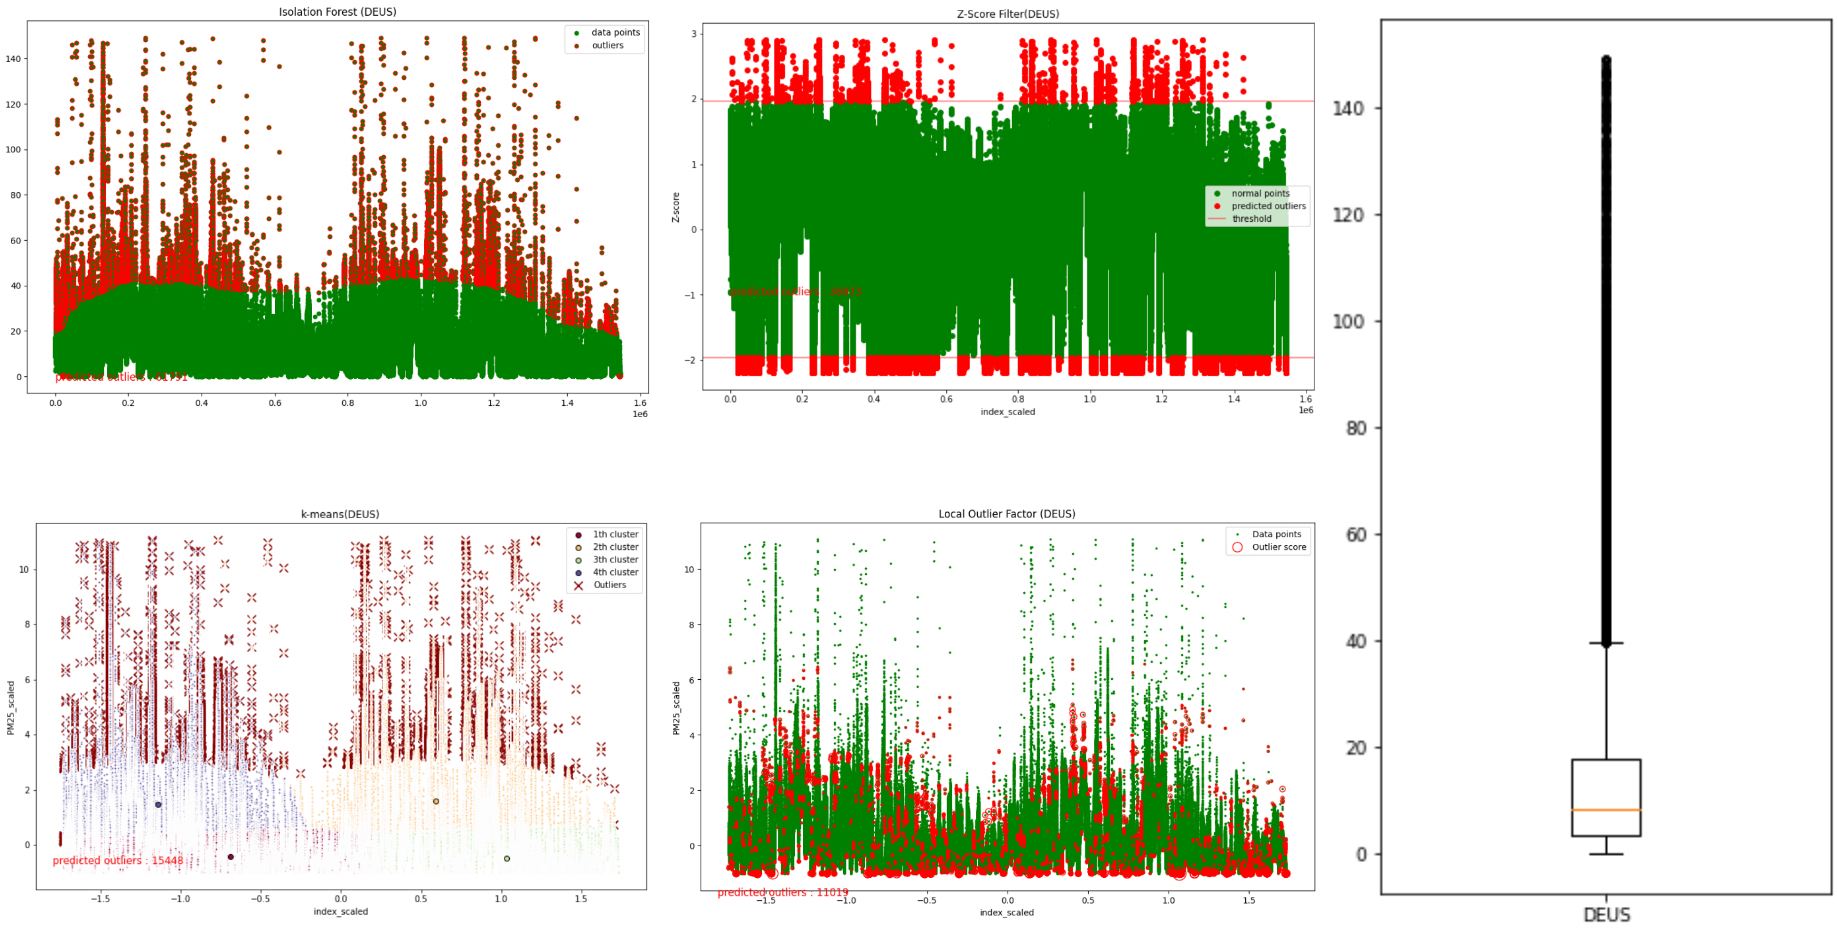
\includegraphics[\linewidth]{images/Visualisierung der Ausreißers.jpg}
            \caption{Visualisierung der Ausreißers}
            \label{fig:Ergebnisse in 2D}
        \end{figure}

        표 1에 의해 iForest, z-Score, IQR과 K-Means Methoden을 이용한 이상치탐지는 모델의 성능에 대한 긍정적인 영향을 보였으며 LOF Methode는 오히려 모델성능에 부정적인 영향을 미쳤습니다. 그 중 iForest Methode가 가장 잘 개선된 모델을 구축했다. 이상치 탐지에 대한 시각적 지표인 표 1.iForest에서 볼 수 있듯이 정상치와 이상치의 경계가 꽤 아름다운 곡선을 만들어 냈다. 수치적 지표로 분석 해보면 이상치제거를 통한 모델의 성능이 2.42\% 더 좋아졌는데 이는 기존의 모델보다 

        LOF Methode에 대한 이러한 부정적 결과는 그림 1.LOF에서 볼 수 있듯이 유의미한 값들이 너무 많이 제거되었기 때문으로 보입니다. 다시말해, 밀집된 지역의 데이터들이 제거되어 이러한 결과를 불러왔다고 볼 수 있습니다. 이는 LOF Methode의 특성으로, 밀도가 낮은 지역의 데이터들만 제거되는 다른 Methoden들과 달리 LOF Methode는 어떤 밀집된 곳에 존재하는 데이터포인트가 해당 지역의 평균 밀도보다 낮을 경우 그 데이터포인트를 제거하기 때문입니다. K-Means Methode 또한 많은 양은 아니지만 몇몇 밀집된 지역에 존재하는 데이터들이 제거됨으로써 다른 iForest, z-Score와 IQR Methode보다 낮은 성능을 보인것으로 판단됩니다. 물론 이 Methode는 무의미한 값들 또한 꽤 많이 제거하였기에 LOF와 달리 모델의 성능을 높인다는 결과를 보였습니다.

        z-Score와 IQR 중에 근소한 차이로 z-Score Methode가 더 좋은 성능을 보였다. 섹션 \ref{sec:Boxplot-Rule}과 \ref{sec:z-Score}에서 기술한 것 처럼 IQR의 Whisker가 1.5일 경우 전체 데이터세트에서 0.7\%를 이상치로 분류하고, z-Score의 Threshold를 1.97로 설정할 경우 전체 데이터세트에서 약 5\%의 데이터가 이상치로 분류된다. 이 Arbeit에서 사용되는 데이터세트는 이상치로 보이는 데이터가 많으므로 전체 데이터세트에서 약 5\%를 제거한 z-Score Methode가 더 좋은 성능을 발휘하였다. 하지만 이 Methode는 IQR보다 약 700\% 더 많은 이상치를 제거했음에도 불구하고 성능은 고작 101\%정도 더 좋아졌는데, 유의미한 값의 제거가 그 이유이다. 실제로 z-Score가 센서 'DEUS'에서 탐지한 36873개의 이상데이터 중에 양의 Threshold 값 이상의 이상데이터는 고작 6143개인 것에 반해 음의 Threshold값 이하의 이상데이터는 무려 30730개이다. 따라서 해당 데이터세트의 경우 낮은 pm값의 제거는 성능의 향상에 도움은 주지만 그 효율이 좋지 않다고 결론내릴 수 있다. 또한 이렇게 제거된 데이터세트를 이용하여 모델을 훈련하고 검증할 경우 해당 모델이 해당 데이터세트에 Underfitting될 가능성이 존재하기 때문에 이러한 이상치 제거는 피해야 할 것으로 보인다.

        iForest의 성능이 가장 좋은 이유를 연역적 방법으로 설명하자면, 밀집된 지역의 데이터를 제거하지도 않았고 너무 적은 양의 데이터를 이상치로 분류하지도 않았으며 낮은 pm값도 제거하지 않았기 때문이라고 할 수 있다. 이는 곧 어떤 데이터세트가 직관적인 관점에서 많은 양의 이상치를 갖고 있다고 판단될 경우 이러한 부분을 주의한다면 최적의 이상치탐지 성능을 얻을 수 있다고 해석할 수 있다.